\documentclass{hyconsys-presentation}

% add extra packages here
%\usepackage{bla_bla_bla}


% add you references in the refs.bib file or replace this
% with another file
\addbibresource{refs.bib}


% add extra new commands here
\newcommand{\B}{\mathbb{B}}
\newcommand{\R}{\mathbb{R}}
\newcommand{\N}{\mathbb{N}}
\newcommand{\Z}{\mathbb{Z}}
\newcommand{\tz}[1]{\times10^{#1}}


\title[]{
  Title of the talk.
}

\author[Running author names]{
	First Author Name\inst{1},
	Second Author Name\inst{2}
}

\institute[]{
	\inst{}\\
	\inst{1}Inst. 1: Department, Institute/University\\
	\inst{2}Inst. 2: Department, Institute/University\\
}

\date{
	\\Event name, 
	\\Talk location/date
}

% comment this if you don't want to have a footer
\footline{\insertshortauthor~|~\insertshorttitle}


\begin{document}
	\setbeamertemplate{caption}{\raggedright\insertcaption\par}

	%-------------------------------------------------------------
	% Title frame
	%-------------------------------------------------------------
	\begin{frame}[noframenumbering]
		\titlepage
	\end{frame}


	%-------------------------------------------------------------
	% Example one column frame
	%-------------------------------------------------------------
	\begin{frame} \frametitle{Example one column frame}
		\begin{columns}
			\begin{column}{0.99\textwidth}
				\textbf{Example subtitle A:}
				\begin{itemize}
					\item item 1.
					\item item 2.
					\item \textbf{item 3.:} 
					\begin{itemize}
						\item subitem 3.1.
						\item subitem 3.2.
					\end{itemize}
				\end{itemize}
				
				\vspace{1em}
				\textbf{Example subtitle B:}
					\textit{
						 "Some quoted example text. Some quoted example text. Some quoted example text. 
						 Some quoted example text. Some quoted example text. Some quoted example text. 
						 Some quoted example text. Some quoted example text. Some quoted example text. 
						 Some quoted example text. Some quoted example text. Some quoted example text. 
						 Some quoted example text. Some quoted example text. Some quoted example text. 
						 Some quoted example text. Some quoted example text. Some quoted example text. 
						 Some quoted example text. Some quoted example text. Some quoted example text. ".									
					}
			\end{column}
		\end{columns}
	\end{frame}

	\begin{frame} \frametitle{Example frame with multiple columns.}
		\begin{columns}
			\begin{column}{0.6\textwidth}				
				\textbf{A column with 60\% width:}
				\begin{itemize}			
					\item Example item.
					\item Example item.
					\item Example item.
					\item Example item.
				\end{itemize}				
			\end{column}
			\begin{column}{0.4\textwidth}
				\textbf{A column with 40\% width:}
				\begin{figure}
					\centering
					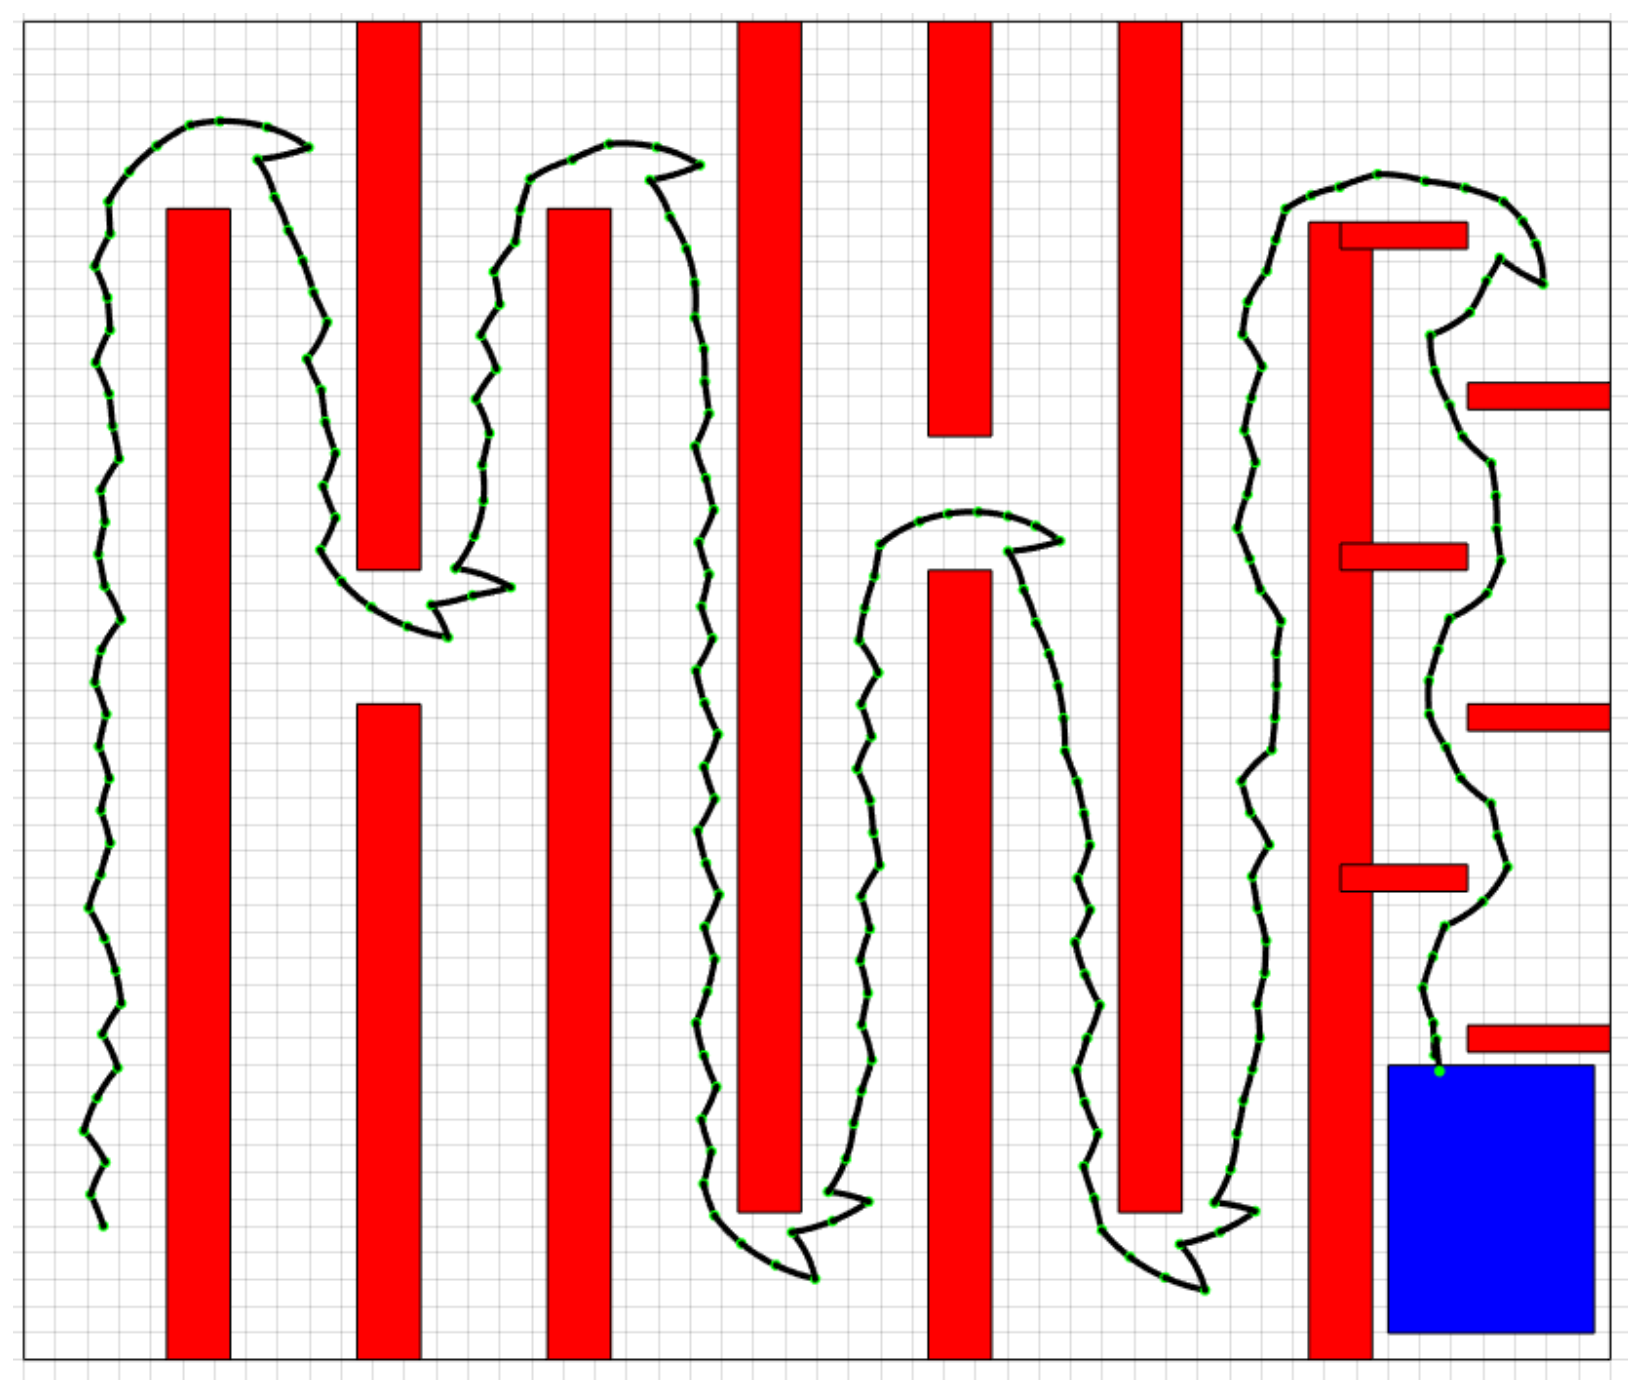
\includegraphics[width=0.50\textwidth]{figures/car_maze.png}
				\end{figure}		    
			\end{column}
		\end{columns}
		
		
		\hspace{-1.2em}
		\textbf{One column just below the two columns:}\\
		\vspace{0.5em}
		Some example text. Some example text. Some example text. Some example text. 
		
	\end{frame}

	% -----------------
	% Final notes, thanks, and ack. frame
	% -----------------
	\begin{frame} \frametitle{Final Notes and Acknowledgments}	
		\begin{columns}
			\begin{column}{0.65\textwidth}	
				
				\vspace{-0.5em}
				\begin{itemize} 
					\item Note 1.
					\item Note 2. 
					\item Note 3.
				\end{itemize}
				
				\vspace{0.5em}
				\textbf{We would like to thank...}
				\begin{itemize}
					\item ... DAAD, ERC, and DFG for funding this work. 
					\item ... anyone else you like to mention.
					\vspace{1em}
					\item \textbf{... and you, for your attention!}
				\end{itemize}
			\end{column}
		
			\begin{column}{0.35\textwidth}				
				\vspace{-5em}				
				\begin{figure}
					\centering
					\includegraphics[width=0.7\textwidth]{figures/DAAD_logo.png}
				\end{figure}	
				\begin{figure}
					\centering
					
\includegraphics[width=0.7\textwidth]{figures/ERC_logo.png}
				\end{figure}
				\begin{figure}
					\centering
					
\includegraphics[width=0.7\textwidth]{figures/DFG_logo.png}
				\end{figure}			
			\end{column}
		\end{columns}							
	\end{frame}


\end{document}

